\documentclass[12pt]{article}

\usepackage{amssymb}
\usepackage{graphicx}
\usepackage{amsmath}
\usepackage[utf8]{inputenc}

\title{Dokumentation "WvD-App"}
\author{JAG}

\begin{document}

\maketitle
\tableofcontents
\setcounter{tocdepth}{3}

\section{Projektidee}

\subsection{Spielbeschreibung}
Thematisch geht es darum, dass das kleine Dörfchen Düsterwald von Werwölfen heimgesucht wird.
Die Gruppe der Bürger versucht die Wölfe, die sich als Bürger getarnt haben, zu entlarven.
Dagegen versuchen die Wölfe als einzige zu überleben und Widersacher auszuschalten.

\subsubsection{Vorbereitung}
Der Spielleiter mischt alle Charakterkarten und teilt an jeden Spieler verdeckt eine davon aus.
Die Spieler schauen sich ihre Karte an und erkennen nun, ob sie einen Werwolf, einen einfachen
Dorfbewohner oder eine Sonderrolle verkörpern. Danach ruft der Spielleiter zur ersten Nacht aus und
das eigentliche Spiel kann beginnen.

\subsubsection{Nachtphase}
In der Nachtphase schließen alle Spieler die Augen. Der Spielleiter ruft die handelnden Charaktere
einzeln auf. Sie öffnen ihre Augen und führen ihre Aktion aus.

Der <Dieb> ist der erste, der im Spiel erwacht. Wird mit Dieb gespielt, werden zwei Karten mehr
ausgeteilt. Der Dieb darf diese ansehen und seine Karte gegen eine der beiden übrig gebliebenen
Karten austauschen. Er hat ab jetzt also eine neue Rolle. Möchte er nicht tauschen, ist er für den
Rest des Spiels einfacher Dorfbewohner.

<Amor> erwacht nur einmal in der allerersten Nacht, um zwei Spieler seiner Wahl miteinander zu
verkuppeln (eventuell auch sich selbst). Danach schläft er wieder ein. Anschließend berührt der
Spielleiter die beiden Verliebten an der Schulter, sodass diese kurz erwachen können und wissen,
wer der jeweilige Partner ist. Die Verliebten haben im Laufe des Spiels die Aufgabe, den Partner
zu beschützen, denn wenn einer der beiden stirbt, macht es ihm der Partner trauernd nach; sie
dürfen nie gegeneinander stimmen.

Werden die <Werwölfe> vom Spielleiter aufgerufen, wachen sie auf und erkennen sich gegenseitig.
Je nach Spielerzahl gibt es zwei bis vier Wölfe.
Die Wölfe einigen sich durch Gesten auf ein Opfer und schlafen dann wieder ein.
Der Spielleiter merkt sich das Opfer der Werwölfe.

Das kleine <Mädchen> darf nachts in der Werwolf-Phase heimlich blinzeln, um so die Werwölfe zu
erkennen. Die Werwölfe ihrerseits hingegen achten natürlich darauf, das Mädchen dabei zu ertappen,
es besteht also beim Blinzeln ein gewisses Risiko.

Die <Seherin> erwacht in der Nacht alleine und zeigt auf einen Spieler.
Der Spielleiter zeigt der Seherin nun die entsprechende Charakter-Karte der Person.
Die Seherin weiß dadurch mehr als die übrigen Dorfbewohner, muss aber mit ihrem Wissen
sorgfältig umgehen, um nicht von den Werwölfen enttarnt zu werden.

Die <Hexe> erwacht immer nachem die Werwölfe ihr Opfer ausgesucht haben.
Sie hat im Verlauf des gesamten Spiels einen Gift- und einen Heiltrank.
Der Spielleiter zeigt auf die Person, die von den Werwölfen als Mordopfer gewählt wurde und die
Hexe kann diese mit ihrem Heiltrank heilen (auch sich selbst), so dass es am nächsten Morgen keinen
Toten gibt. Sie kann aber auch den Gifttrank auf einen anderen Spieler anwenden -
dann gibt es mehrere Tote.

Scheidet der <Jäger> aus dem Spiel aus, feuert er in seinem letzten Atemzug noch einen Schuss ab,
mit dem er einen Spieler seiner Wahl mit in den Tod reißt, d.h. er bestimmt einen Spieler,
der mit ihm aus dem Spiel ausscheidet.

\subsubsection{Tagphase}
Am Tag wachen alle Spieler auf. Das Opfer der Werwölfe wird verkündet, es dreht seine Karte um,
gilt als tot und scheidet aus der Runde aus, d. h., er darf keinen Kommentar zum Spiel mehr abgeben.
Nun diskutieren die Dorfbewohner, wer von ihnen ein Werwolf sein könnte. Diese Diskussionsphase
ist das eigentliche Herzstück des Spiels.

Am Ende des Tages gibt es eine sogenannte Abstimmung durch das Dorfgericht, wobei auf Kommando des
Spielleiters jeder, außer den ausgeschiedenen Personen, mit dem Finger auf eine für ihn verdächtige
Person deutet. Wer die meisten Stimmen erhält, scheidet aus. Bei Gleichstand gibt es eine Stichwahl,
bei erneutem Patt entscheidet ein zu Spielbeginn gewählter Hauptmann. Den verbleibenden Spielern
wird die Charakterrolle des ausgeschiedenen Spielers bekanntgeben. Nach dem Tag wird es wieder
Nacht und der Zyklus beginnt von vorn.

\subsubsection{Ende des Spiels}
Das Spiel endet, sobald entweder alle Werwölfe oder alle Bürger tot sind.
Das Ziel der Werwölfe ist es, alle Bürger auszulöschen, während die Dorfbewohner den Wölfen den
Garaus machen wollen. Lediglich wenn das Liebespaar aus einem Werwolf und einem Dorfbewohner besteht,
können diese beiden Spieler nur dann gewinnen, wenn außer ihnen niemand überlebt.

\subsection{Idee: Umsetzung als Android-App}

\section{Umsetzung}

	\subsection{Projektplanung}
		\subsubsection{Meilensteine}
		\subsubsection{Projektplan}
		\subsubsection{Burn-Down-Chart}

	\subsection{Projektdurchführung}
		\subsubsection{Architekturdiagramm}
		\subsubsection{Beschreibung der Klassen}
		siehe documentation.txt
		
\subsubsection{Datenbankschema}
		
\begin{figure}[] 
  \centering
     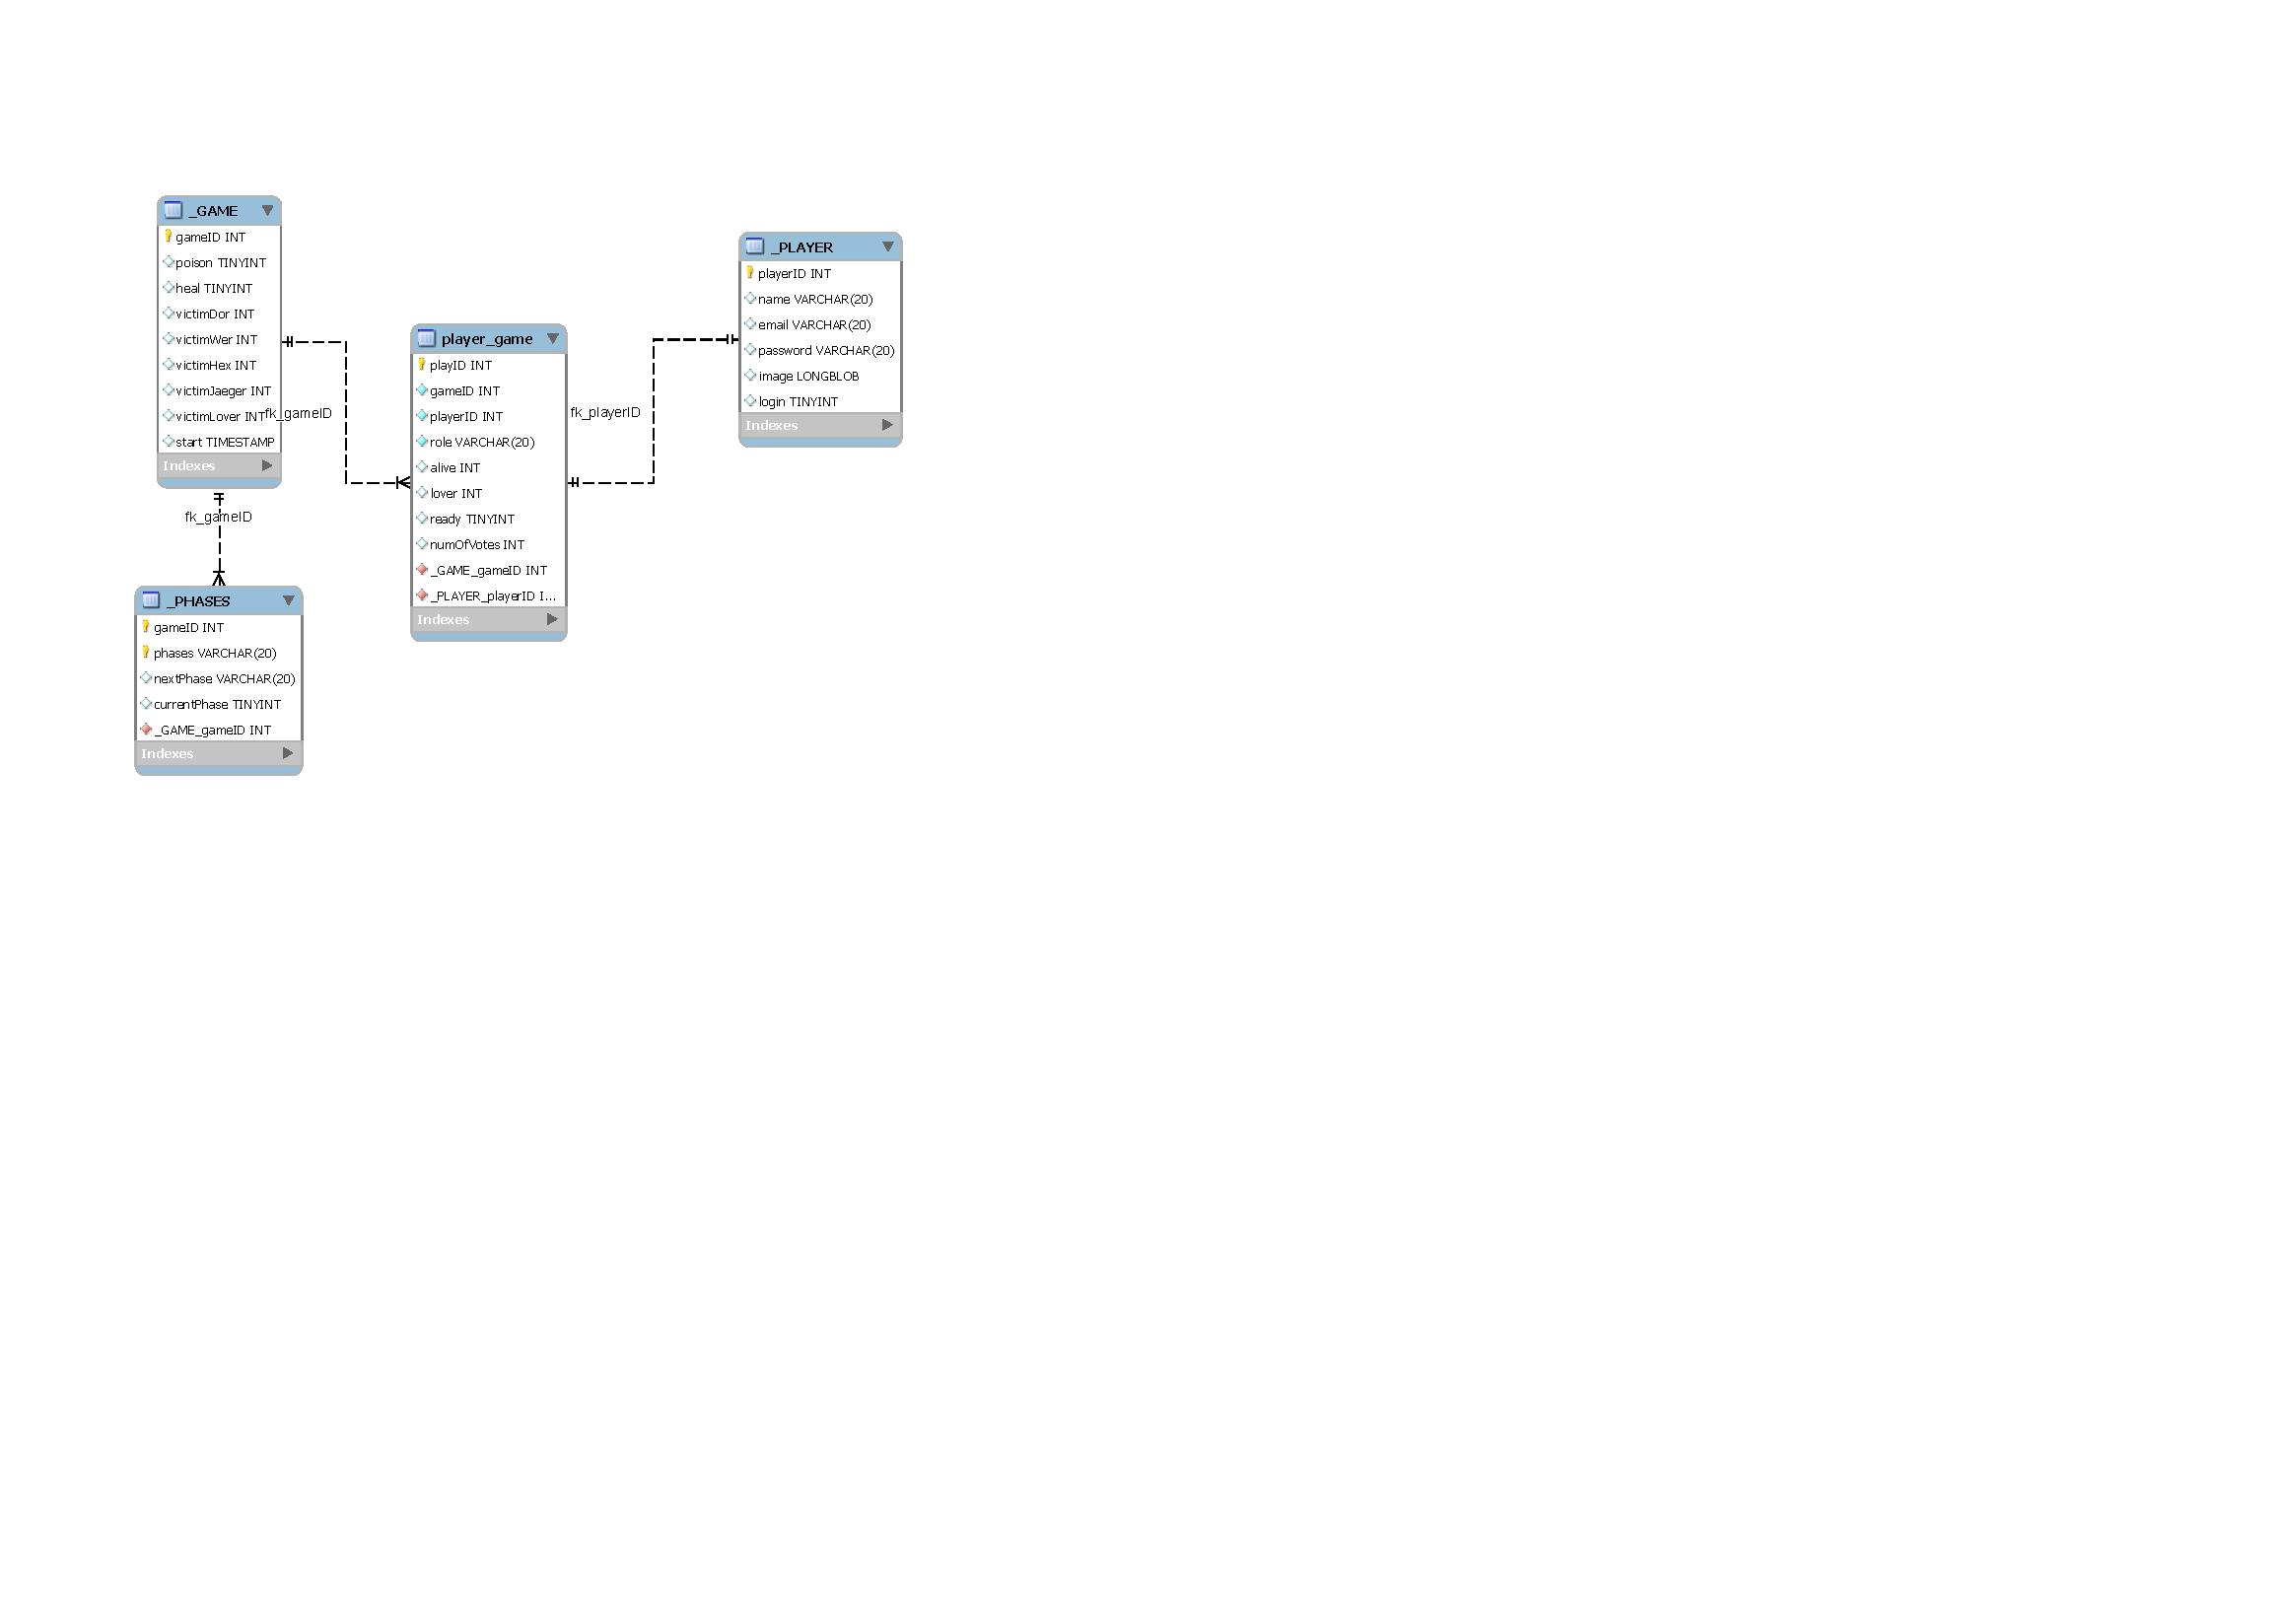
\includegraphics[height = 9 cm, width = 12cm]{DB_Schema}
  \caption{Datenbankschema}
\end{figure}
	

\textbf{$player\_game.$}
Diese Tabelle ordnet einem Spieler ein Spiel zu und speichert, welche Rolle dieser verkörpert (\textit{role}). Der \textit{ready}-Wert ist für den Beginn des Spiels gedacht. Sobald alle Spieler dem Spiel beigetreten und bereit sind (\textit{ready == 1}) beginnt das Spiel. $ \textit{"Erklärung:numOfVotes"} $
\\

\textbf{$\_GAME.$}
In dieser Tabelle werden Spiel-spezifische Informationen gespeichert. Sie enthält den Tränke-Vorrat der Hexe (\textit{poison, heal}) und die aktuell zum Tode verurteilten (\textit{victimDor, victimWer, ...}).
\\

\textbf{$\_PHASES.$}
Hier werden zu jedem Spiel die notwendigen Spielphasen gespeichert. Abhängig von der Auswahl der Rollen werden diese zu Beginn des Spiels festgelegt. Die Tabelle zeigt die jeweiligen Phasen (\textit{phases}) mit ihren darauf folgenden Phasen (\textit{nextPhase}). Der Wert \textit{currentPhase} gibt an, in welcher Phase sich ein Spiel befindet.
\\

\textbf{$\_PLAYER.$}
Diese Tabelle enthält alle Spieler-Accounts. Der \textit{login}-Wert gibt an, ob ein Spieler auf einem Gerät angemeldet ist. So wird sicher gestellt, dass jeder Spieler nur auf einem Gerät angemeldet sein kann.  


\end{document}

